\documentclass[DaoFP]{subfiles}
\begin{document}
    \setcounter{chapter}{15}

    \chapter{Comonads\text{(余单子)}}

    如果它的发音更容易,我们可能会将副作用称为“ntext”,因为副作用的对偶是“context”(上下文)。

    就像我们使用Kleisli箭头来处理副作用一样,我们使用co-Kleisli箭头来处理上下文。

    让我们从一个熟悉的例子开始,即将环境作为上下文。我们之前通过对箭头进行柯里化构造了一个Reader Monad(读取器单子):
    \begin{haskell}
    (a, e) -> b
    \end{haskell}
    然而,这次我们将其视为一个co-Kleisli箭头,它是一个来自“上下文化”参数的箭头。

    与单子类似,我们也对co-Kleisli箭头的组合感兴趣。对于携带环境的箭头来说,这相对容易:
    \begin{haskell}
        composeWithEnv :: ((b, e) -> c) -> ((a, e) -> b) -> ((a, e) -> c)
        composeWithEnv g f = \(a, e) -> g (f (a, e), e)
    \end{haskell}

    实现一个在这种组合下作为身份的箭头也很简单:
    \begin{haskell}
        idWithEnv :: (a, e) -> a
        idWithEnv (a, e) = a
    \end{haskell}

    这强烈暗示存在一个类别,在这个类别中co-Kleisli箭头作为态射。

    \begin{exercise}
        证明使用\hask{composeWithEnv}的co-Kleisli箭头的组合是结合的。
    \end{exercise}

    \section{Comonads in Programming\text{(编程中的余单子)}}

    如果一个函子\hask{w}(可以看作是一个风格化的倒置\hask{m})支持co-Kleisli箭头的组合,那么它就是一个余单子:

    \begin{haskell}
        class Functor w => Comonad w where
        (=<=) :: (w b -> c) -> (w a -> b) -> (w a -> c)
        extract :: w a -> a
    \end{haskell}

    这里,组合以中缀操作符的形式书写。组合的单位被称为\hask{extract},因为它从上下文中提取一个值。

    让我们尝试使用我们的例子。将环境作为对的第一个组件传递是方便的。然后,余单子由对构造器\hask{((,) e)}的部分应用给出。
    \begin{haskell}
        instance Comonad ((,) e) where
        g =<= f = \ea -> g (fst ea, f ea)
        extract = snd
    \end{haskell}

    与单子一样,co-Kleisli组合可以用于无点风格的编程。但我们也可以使用\hask{join}的对偶,称为\hask{duplicate}:
    \begin{haskell}
        duplicate :: w a -> w (w a)
    \end{haskell}
    或者使用\hask{bind}的对偶,称为\hask{extend}:
    \begin{haskell}
        extend :: (w a -> b) -> w a -> w b
    \end{haskell}
    下面是如何用\hask{duplicate}和\hask{fmap}来实现co-Kleisli组合的:
    \begin{haskell}
        g =<= f = g . fmap f . duplicate
    \end{haskell}
    \begin{exercise}
        实现\hask{duplicate}和\hask{extend}之间的互相转换。
    \end{exercise}
    \subsection{The \hask{Stream} Comonad\text{(流余单子)}}
    余单子处理更大规模,有时是无限的上下文的例子很有趣。这里有一个无限流:
    \begin{haskell}
        data Stream a = Cons a (Stream a)
        deriving Functor
    \end{haskell}

    如果我们将这样的流视为类型\hask{a}的值在一个无限尾部的上下文中,我们可以为它提供一个\hask{Comonad}实例:
    \begin{haskell}
        instance Comonad Stream where
        extract (Cons a as) = a
        duplicate (Cons a as) = Cons (Cons a as) (duplicate as)
    \end{haskell}
    这里,\hask{extract}返回流的头部,而\hask{duplicate}将一个流变成一个流的流,在这个流中,每一个连续的流都是前一个的尾部。

    直观上,\hask{duplicate}为迭代设置了舞台,但它以非常通用的方式进行。每个子流的头部可以解释为原始流中的未来“当前位置”。

    这使得进行一个遍历这些流头部的计算变得容易。但这并不是余单子的力量所在。它让我们能够进行需要任意前瞻的计算。这种计算不仅需要访问连续子流的头部,还需要访问它们的尾部。

    这就是\hask{extend}的作用:它将给定的co-Kleisli箭头\hask{f}应用于由\hask{duplicate}生成的所有流:
    \begin{haskell}
        extend f (Cons a as) = Cons (f (Cons a as)) (extend f as)
    \end{haskell}

    这里有一个计算流前五个元素平均值的co-Kleisli箭头的例子:
    \begin{haskell}
        avg :: Stream Double -> Double
        avg  = (/5). sum . stmTake 5
    \end{haskell}
    它使用了一个帮助函数,该函数提取前\hask{n}个元素:
    \begin{haskell}
        stmTake :: Int -> Stream a -> [a]
        stmTake 0 _ = []
        stmTake n (Cons a as) = a : stmTake (n - 1) as
    \end{haskell}

    我们可以使用\hask{extend}在整个流上运行\hask{avg}来平滑局部波动。电气工程师可能会将其识别为一个简单的\index{low-pass filter}\text{低通滤波器},其中\hask{extend}实现了\index{convolution}\text{卷积}。它生成了原始流的一个滑动平均值。
    \begin{haskell}
        smooth :: Stream Double -> Stream Double
        smooth = extend avg
    \end{haskell}

    余单子对于结构化计算在空间上或时间上扩展的数据结构中很有用。这些计算足够局部以定义“当前位置”,但需要从邻近位置收集信息。信号处理或图像处理是很好的例子。模拟,在这些模拟中,微分方程必须在体积内迭代求解:气候模拟、宇宙学模型或核反应等等。康威的生命游戏也是一个很好的余单子方法测试场。

    有时在连续的数据流上进行计算是方便的,推迟采样直到最后一步。这里是一个信号的例子,它是时间的函数(由\hask{Double}表示):
    \begin{haskell}
        data Signal a = Sig (Double -> a) Double
    \end{haskell}
    第一个组件是由时间函数实现的连续\hask{a}流。第二个组件是当前时间。

    这是连续流的\hask{Comonad}实例:
    \begin{haskell}
        instance Comonad Signal where
        extract (Sig f x) = f x
        duplicate (Sig f x) = Sig (\y -> Sig f (x - y)) x
        extend g (Sig f x) = Sig (\y -> g (Sig f (x - y))) x
    \end{haskell}
    这里,\hask{extend}将滤波器\hask{g :: Signal a -> a}卷积到整个流上。

    \begin{exercise}
        为双向流实现\hask{Comonad}实例:
        \begin{haskell}
            data BiStream a = BStr [a] [a]
        \end{haskell}
        假设两个列表都是无限的。提示:将第一个列表视为过去(逆序);将第二个列表的头部视为现在,其尾部视为未来。
    \end{exercise}

    \begin{exercise}
        为之前练习中的\hask{BiStream}实现低通滤波器。它在三个值上进行平均:当前值、立即过去的一个值和立即未来的一个值。对于电气工程师:实现一个高斯滤波器。
    \end{exercise}

    \section{Comonads Categorically\text{(范畴论中的余单子)}}

    我们可以通过反转单子定义中的箭头来获得余单子的定义。我们的\hask{duplicate}对应于反转的\hask{join},而\hask{extract}是反转的\hask{return}。

    因此,余单子是一个配备了两个自然变换的自函子$W$:
\begin{align*}
\delta &\colon W \to W \circ W \\
\varepsilon &\colon W \to \text{Id}
\end{align*}

这些变换(分别对应\hask{duplicate}和\hask{extract})必须满足与单子相同的恒等式,只不过箭头是反转的。

这些是余单子的余单元定律:
\[
\begin{tikzcd}
\text{Id} \circ W
\arrow[rrd, "="']
& & W \circ W
\arrow[ll, "\varepsilon \circ W"']
\arrow[rr, "W \circ \varepsilon"]
&& W \circ \text{Id}
\arrow[lld, "="]
\\
&& W
\arrow[u, "\delta"]
\end{tikzcd}
\]
这就是结合律:
\[
\begin{tikzcd}
(W \circ W) \circ W
\arrow[rr, "="]
&&
W \circ (W \circ W)
\\
W \circ W
\arrow[u, "\delta \circ W"]
& & W \circ W
\arrow[u, "W \circ \delta"']
\\
&  W
\arrow[ul, "\delta"]
\arrow[ur, "\delta"']
\end{tikzcd}
\]

\subsection{Comonoids\text{(余半群)}}

我们已经看到了单子定律如何从半群定律中得出。我们可以期望余单子定律应当来自半群的对偶版本。

确实,一个\index{comonoid}\text{余半群}是一个对象$w$,它在一个单元范畴$(\mathcal{C}, \otimes, I)$中配备了两个称为余乘法和余单元的态射:
\begin{align*}
\delta &\colon w \to w \otimes w \\
\varepsilon &\colon w \to I
\end{align*}
我们可以用自函子的复合替换张量积,用恒等函子替换单位对象,以获得作为自函子类别中的余半群的余单子定义。

在Haskell中,我们可以为笛卡尔积定义\hask{Comonoid}类型类:
\begin{haskell}
class Comonoid w where
split   :: w -> (w, w)
destroy :: w -> ()
\end{haskell}

与它们的兄弟monoids(单半群)相比,comonoids(余半群)谈论较少,主要是因为它们被视为理所当然。在笛卡尔范畴中,每个对象都可以通过使用对角线映射$\Delta_a \colon a \to a \times a$来进行余乘法,并使用到终对象的唯一箭头来进行余单元,从而成为一个comonoid。

在编程中,这是我们不加思索就会做的事情。余乘法意味着能够复制一个值,余单元意味着能够放弃一个值。

在Haskell中,我们可以轻松地为任何类型实现\hask{Comonoid}实例:
\begin{haskell}
instance Comonoid w where
split w   = (w, w)
destroy w = ()
\end{haskell}
事实上,我们在使用函数的参数两次或根本不使用它时根本不会多想。但如果我们想要明确,我们可以将这样的函数:
\begin{haskell}
f x = x + x
g y = 42
\end{haskell}
写成:
\begin{haskell}
f x = let (x1, x2) = split x
in x1 + x2
g y = let () = destroy y
in 42
\end{haskell}

然而,在某些情况下,复制或丢弃变量是不合适的。这种情况出现在参数是外部资源(例如文件句柄、网络端口或在堆上分配的内存块)时。这些资源应具有明确的生命周期,从分配到释放。追踪可以轻松复制或丢弃的对象的生命周期是非常困难的,并且是编程错误的一个著名来源。

基于笛卡尔范畴的编程模型将始终存在此问题。解决方案是改用不支持对象复制或销毁的单元(闭)范畴。这样的范畴是\index{linear types}\text{线性类型}的自然设置。在线性类型中,元素被用在\index{Rust}\text{Rust}中,并且在写作本文时,正在尝试在Haskell中使用。在C++中,有一些结构可以模仿线性,例如\hask{unique_ptr}和移动语义。

\section{Comonads from Adjunctions\text{(从伴随构造余单子)}}

我们已经看到,两个函子$L \colon \mathcal{D} \to \mathcal{C}$和$R \colon \mathcal{C} \to \mathcal{D}$之间的伴随$L \dashv R$会产生一个单子$R \circ L \colon \mathcal{D} \to \mathcal{D}$。另一个复合$L \circ R$,它是$\mathcal{C}$中的一个自函子,结果是一个余单子。

伴随的余单元成为余单子的余单元。这可以通过以下弦图来说明:
\[
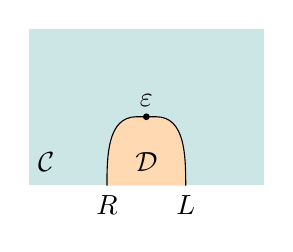
\begin{tikzpicture}
\def\xleft{0.5};
\def\xmid{1};
\def\xright{1.5};

\def \ybot{0};
\def \ymid{1};
\def \ytop{2 * \ymid};
%\def \yt{2 * \ymid - 0.3};
\def \yb{2 * \ybot + 0.3};

\node [below] (a) at (\xleft, \ybot) {$R$};
\node(b) [below] at (\xmid, \ymid) {};
\node[below] (c) at (\xright, \ybot) {$L$};

\filldraw[fill=blue!50!green!20, draw=white] (\xleft-1, \ytop) rectangle (\xright+1, \ybot);

\draw [fill=orange!30] (a.north) to [out=90, in=180] (b.west) -- (b.east) to [out=0, in=90] (c.north);

\filldraw[black] (b) circle (1 pt);
\node [above] at (b) {$\varepsilon$};

\node(l)[right] at (\xleft-1, \yb) {$\mathcal{C}$};
\node(r) at (\xmid, \yb) {$\mathcal{D}$};

\end{tikzpicture}
\]

余乘法由$\eta$的whiskering(缠绕)给出:
\[ \delta = L  \circ \eta \circ R \]
如下弦图所示:
\[
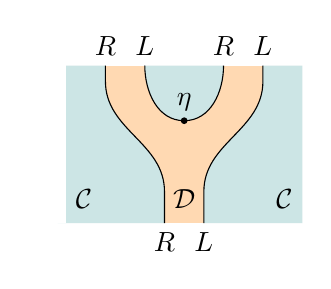
\begin{tikzpicture}
\def \xmid          {0};
\def \xr               {0.5};
\def \xrr             {1}
\def \xrm            {0.25}
\def \xrightmost {1.5}
\def \xl {-\xr}
\def \xll {-\xrr}
\def \xlm {-\xrm}
\def \xleftmost {-\xrightmost}

\def \ybot           {0};
\def \ymidbot     {-0.20};
\def \yeps          {-0.7};
\def \ymid          {-1};
\def \ymidtop     {-1.60}
\def \ytop           {-2};
\def \ylabel        {\ytop + 0.3};
% functors
\node [below] at (\xlm, \ytop)  {$R$};
\node [below] at (\xrm, \ytop) {$L$};

\node [above] at (\xll, \ybot) {$R$};
\node [above] at (\xl, \ybot) {$L$};
\node [above] at (\xr, \ybot) {$R$};
\node [above] at (\xrr, \ybot) {$L$};

\filldraw[fill=orange!30, draw=white] (\xleftmost, \ytop) rectangle (\xrightmost, \ybot);

% left area
\path [fill=blue!50!green!20] (\xleftmost, \ybot) to  (\xll, \ybot) to (\xll, \ymidbot) [out=-90, in=90] to (\xlm, \ymidtop) to  (\xlm, \ytop) to [out=180, in=180] (\xleftmost, \ytop);
% right area
\path [fill=blue!50!green!20] (\xrightmost, \ybot) to (\xrr, \ybot) to (\xrr, \ymidbot) [out=-90, in=90] to (\xrm, \ymidtop) to (\xrm, \ytop) to [out=0, in=180]  (\xrightmost, \ytop);
% cap
\draw [fill=blue!50!green!20] (\xl, \ybot) to [out=-90, in=180] (\xmid, \yeps) to [out=0, in=-90] (\xr, \ybot);
% left curve
\draw (\xll, \ybot) to (\xll, \ymidbot) [out=-90, in=90] to (\xlm, \ymidtop) to  (\xlm, \ytop);
% right curve
\draw (\xrr, \ybot) to (\xrr, \ymidbot) [out=-90, in=90] to (\xrm, \ymidtop) to (\xrm, \ytop);
% eta
\filldraw [black] (\xmid, \yeps) circle (1 pt);
\node [above] at (\xmid, \yeps) {$\eta$};
% categories
\node [right] at (\xleftmost, \ylabel) {$\mathcal{C}$};
\node           at (\xmid, \ylabel)        {$\mathcal{D}$};
\node [left]   at (\xrightmost, \ylabel) {$\mathcal{C}$};

\end{tikzpicture}
\]

与之前一样,余单子定律可以从三角恒等式中导出。

\subsection{Costate Comonad\text{(余状态余单子)}}

我们已经看到,State Monad(状态单子)可以从乘积与指数之间的柯里化伴随构造中生成。左函子被定义为与某个固定对象$s$的乘积:
\[ L_s a = a \times s \]
右函子是以相同对象$s$为参数的指数:
\[ R_s c = c^s \]
组合$L_s \circ R_s$生成一个称为\index{costate comonad}\text{余状态余单子}或\index{store comonad}\text{存储余单子}的余单子。

在Haskell中,右函子将函数类型\hask{s->c}分配给\hask{c},而左函子将\hask{c}与\hask{s}配对。复合的结果是自函子:
\begin{haskell}
data Store s c = St (s -> c) s
\end{haskell}
或者,使用GADT表示法:
\begin{haskell}
data Store s c where
St :: (s -> c) -> s -> Store s c
\end{haskell}
函子实例通过后组合函数到\hask{Store}的第一个组件来实现:
\begin{haskell}
instance Functor (Store s) where
fmap g (St f s) = St (g . f) s
\end{haskell}

这个伴随的余单元成为余单子的\hask{extract},即函数应用:
\begin{haskell}
extract :: Store s c -> c
extract (St f s) = f s
\end{haskell}
这个伴随的单位是自然变换$\eta \colon \text{Id} \to R_s \circ L_s$。我们已经使用它作为状态单子的\hask{return}。这是它在\hask{c}处的分量:
\begin{haskell}
unit :: c -> (s -> (c, s))
unit c = \s -> (c, s)
\end{haskell}
要得到\hask{duplicate},我们需要将$\eta$进行缠绕:
\[ \delta = L_s  \circ \eta \circ R_s \]
缠绕在右边意味着使用\hask{eta}在对象$R_s c$上的分量,而缠绕在左边意味着使用$L_s$来提升此分量。由于Haskell翻译缠绕是一个棘手的过程,我们一步步分析。

为了简单起见,让我们将类型\hask{s}固定为\hask{Int}。我们将左函子封装在一个\hask{newtype}中:
\begin{haskell}
newtype Pair c = P (c, Int)
deriving Functor
\end{haskell}
并保持右函子为类型同义词:
\begin{haskell}
type Fun c = Int -> c
\end{haskell}
伴随的单位可以写成使用显式\hask{forall}的自然变换:
\begin{haskell}
eta :: forall c. c -> Fun (Pair c)
eta c = \s -> P (c, s)
\end{haskell}

我们现在可以实现余乘法作为\hask{eta}的缠绕。在右侧的缠绕通过使用\hask{eta}在\hask{Fun c}上的分量来编码,而在左侧的缠绕通过使用\hask{Pair}函子的\hask{fmap}来提升此分量。我们使用语言扩展\hask{TypeApplications}使其明确使用哪个\hask{fmap}:
\begin{haskell}
delta :: forall c. Pair (Fun c) -> Pair (Fun (Pair (Fun c)))
delta = fmap @Pair eta
\end{haskell}
这可以更明确地重写为:
\begin{haskell}
delta (P (f, s)) = P (\s' -> P (f, s'), s)
\end{haskell}

因此,\hask{Comonad}实例可以写成:
\begin{haskell}
instance Comonad (Store s) where
extract (St f s) = f s
duplicate (St f s) = St (St f) s
\end{haskell}

存储余单子是一个有用的编程概念。为了理解它,让我们再次考虑\hask{s}为\hask{Int}的情况。

我们将\hask{Store Int c}的第一个组件,函数\hask{f :: Int -> c},解释为一个虚拟的无限值流的访问器,每个整数对应一个值。

第二个组件可以解释为当前索引。确实,\hask{extract}使用这个索引来检索当前值。

有了这个解释,\hask{duplicate}生成一个无限流的流,每个流都由不同的偏移量进行移位,而\hask{extend}则对这个流进行卷积。当然,惰性保存了问题:只有我们明确要求的值才会被计算。

还要注意到,我们之前的\hask{Signal}余单子的例子也可以通过\hask{Store Double}复现。

\begin{exercise}
使用存储余单子实现一个元胞自动机。这是描述规则110的co-Kleisli箭头:
\begin{haskell}
step :: Store Int Cell -> Cell
step (St f n) =
case (f (n-1), f n, f (n+1)) of
(L, L, L) -> D
(L, D, D) -> D
(D, D, D) -> D
_ -> L
\end{haskell}
一个元胞可以是活的也可以是死的:
\begin{haskell}
data Cell = L | D
deriving Show
\end{haskell}
运行此自动机的几代。提示:使用Prelude中的\hask{iterate}函数。
\end{exercise}

\subsection{Comonad Coalgebras\text{(余单子余代数)}}

与单子代数对偶,我们有余单子余代数。给定一个余单子$(W, \varepsilon, \delta)$,我们可以构造一个余代数,它由一个承载对象$a$和一个箭头$\phi \colon a \to W a$组成。为了使这个余代数能够与余单子很好地组合,我们要求能够提取用$\phi$注入的值;并且$\phi$作用于$\phi$结果上的提升与重复相同:
\[
\begin{tikzcd}
a
& W a
\arrow[l, "\varepsilon_a"']
\\
& a
\arrow[ul, "id_a"]
\arrow[u, red, "\phi"']
\end{tikzcd}
\hspace{30pt}
\begin{tikzcd}
W(W a)
&W a
\arrow[l, red, "W \phi "']
\\
W a
\arrow[u, "\delta_a"']
& a
\arrow[l, red, "\phi"']
\arrow[u, red, "\phi"']
\end{tikzcd}
\]

与单子代数一样,余单子余代数形成一个类别。给定$\mathcal{C}$中的余单子$(W, \varepsilon, \delta)$,它的余单子余代数形成一个类别,称为Eilenberg-Moore范畴(有时前缀为co-)$\mathcal{C}^W$。

有一个co-Kleisli子范畴$\mathcal{C}^W$,记为$\mathcal{C}_W$。

给定一个余单子$W$,我们可以使用$\mathcal{C}^W$或$\mathcal{C}_W$构造一个伴随构造,复现余单子$W$。这个构造与单子的完全类比。

\subsection{Lenses\text{(透镜)}}

Store余单子的余代数特别有趣。我们先做一些重命名。让我们称载体为\hask{s},状态为\hask{a}。
\begin{haskell}
data Store a s = St (a -> s) a
\end{haskell}
余代数由一个函数给出:
\begin{haskell}
phi :: s -> Store a s
\end{haskell}
它等价于一对函数:
\begin{haskell}
set :: s -> a -> s
get :: s -> a
\end{haskell}
这样一对被称为透镜:\hask{s}称为源,\hask{a}为焦点。

在这种解释下,\hask{get}让我们提取焦点,而\hask{set}则用新值替换焦点以生成一个新的\hask{s}。

透镜最初被引入以描述数据库记录中数据的检索和修改。然后,它们在处理数据结构时得到了应用。透镜客观化了对一个更大对象的部分进行读写访问的思想。例如,透镜可以聚焦于对的一部分或记录的一个特定组件。我们将在下一章讨论透镜和光学。

让我们将余单子余代数的定律应用于透镜。为简单起见,让我们省略方程中的数据构造函数。我们得到以下简化定义:
\begin{haskell}
phi s = (set s, get s)
epsilon (f, a) = f a
delta (f, a) = (\x -> (f, x), a)
\end{haskell}

\[
\begin{tikzcd}
s
& W s
\arrow[l, "\varepsilon_s"']
\\
& a
\arrow[ul, "id_s"]
\arrow[u, red, "\phi"']
\end{tikzcd}
\hspace{30pt}
\begin{tikzcd}
W(W s)
&W s
\arrow[l, red, "W \phi "']
\\
W s
\arrow[u, "\delta_s"']
& s
\arrow[l, red, "\phi"']
\arrow[u, red, "\phi"']
\end{tikzcd}
\]

第一个定律告诉我们,应用\hask{get}的结果来应用\hask{set}的结果是恒等的:
\begin{haskell}
set s (get  s) = s
\end{haskell}
这被称为透镜的set/get定律。当你用相同的焦点替换焦点时,不应改变任何东西。

第二个定律需要将\hask{fmap phi}应用于\hask{phi}的结果:
\begin{haskell}
fmap phi (set s, get s) = (phi . set s, get s)
\end{haskell}
这应该等同于应用\hask{delta}:
\begin{haskell}
delta (set s, get s) = (\x -> (set s, x), get s)
\end{haskell}
比较两者,我们得到:
\begin{haskell}
phi . set s = \x -> (set s, x)
\end{haskell}
让我们将其应用于某个\hask{a}:
\begin{haskell}
phi (set s a) = (set s, a)
\end{haskell}
使用\hask{phi}的定义,我们得到:
\begin{haskell}
(set (set s a), get (set s a)) = (set s, a)
\end{haskell}
我们有两个等式。第一个组件是函数,所以我们将它们应用于某个\hask{a'},得到set/set透镜定律:
\begin{haskell}
set (set s a) a' = set s a'
\end{haskell}
将焦点设置为\hask{a},然后将其覆盖为\hask{a'}与直接将焦点设置为\hask{a'}是相同的。

第二个组件给我们get/set定律:
\begin{haskell}
get (set s a) = a
\end{haskell}
在我们将焦点设置为\hask{a}后,\hask{get}的结果是\hask{a}。

满足这些定律的透镜被称为\index{lawful lenses}\text{合法透镜}。它们是存储余单子的余代数。

\end{document}
